% !TeX program = xelatex
\documentclass[12pt, a4paper]{article}
\usepackage{amsmath}
\usepackage{xeCJK}
\usepackage{amsmath}
\usepackage{amssymb}
\usepackage{xcolor}
\usepackage{parskip}
\usepackage{tikz}
\usepackage{enumitem}

\setmainfont{Latin Modern Roman}
\setCJKmainfont{Noto Serif CJK TC}

\title{MOSFET}

\begin{document}
\section*{Concept of MOSFET}
\textbf{NMOS Transistor} \\
\begin{center}
	

\tikzset{every picture/.style={line width=0.75pt}} %set default line width to 0.75pt        

\begin{tikzpicture}[x=0.75pt,y=0.75pt,yscale=-1,xscale=1]
%uncomment if require: \path (0,300); %set diagram left start at 0, and has height of 300

%Shape: Rectangle [id:dp41184659712713045] 
\draw   (208,137.4) -- (460.82,137.4) -- (460.82,249.37) -- (208,249.37) -- cycle ;
%Curve Lines [id:da1594417897959518] 
\draw    (220.4,137.6) .. controls (221.82,178.34) and (214.49,184.34) .. (256.49,183.67) .. controls (298.49,183.01) and (263.15,159.67) .. (332.49,159.67) .. controls (401.82,159.67) and (369.15,184.34) .. (410.49,183.67) .. controls (451.82,183.01) and (446.49,167.67) .. (447.82,137.01) ;
%Rounded Same Side Corner Rect [id:dp5871139863434869] 
\draw  [fill={rgb, 255:red, 0; green, 0; blue, 0 }  ,fill opacity=0.26 ] (276.49,155.81) .. controls (276.49,158.31) and (274.46,160.34) .. (271.95,160.34) -- (236.3,160.34) .. controls (233.8,160.34) and (231.77,158.31) .. (231.77,155.81) -- (231.77,137.67) .. controls (231.77,137.67) and (231.77,137.67) .. (231.77,137.67) -- (276.49,137.67) .. controls (276.49,137.67) and (276.49,137.67) .. (276.49,137.67) -- cycle ;
%Rounded Same Side Corner Rect [id:dp4186792611324751] 
\draw  [fill={rgb, 255:red, 0; green, 0; blue, 0 }  ,fill opacity=0.26 ] (438.49,155.81) .. controls (438.49,158.31) and (436.46,160.34) .. (433.95,160.34) -- (398.3,160.34) .. controls (395.8,160.34) and (393.77,158.31) .. (393.77,155.81) -- (393.77,137.67) .. controls (393.77,137.67) and (393.77,137.67) .. (393.77,137.67) -- (438.49,137.67) .. controls (438.49,137.67) and (438.49,137.67) .. (438.49,137.67) -- cycle ;
%Shape: Rectangle [id:dp32485593490259146] 
\draw  [fill={rgb, 255:red, 74; green, 144; blue, 226 }  ,fill opacity=0.27 ] (276.49,137.67) -- (393.82,137.67) -- (393.82,146.34) -- (276.49,146.34) -- cycle ;
%Shape: Rectangle [id:dp01815798269034341] 
\draw  [fill={rgb, 255:red, 0; green, 0; blue, 0 }  ,fill opacity=0.7 ] (276.49,125.67) -- (394.49,125.67) -- (394.49,137.67) -- (276.49,137.67) -- cycle ;
%Straight Lines [id:da06452216641956743] 
\draw    (302.87,91.81) -- (316.87,91.78) ;
%Straight Lines [id:da6999367673807005] 
\draw    (305.43,94) -- (314.03,93.96) ;
%Straight Lines [id:da18572591301865693] 
\draw    (308.37,96.26) -- (311.19,96.22) ;

%Straight Lines [id:da4312597473302121] 
\draw    (296.01,74.23) -- (324.28,74.1) ;
%Straight Lines [id:da6309967999788484] 
\draw    (301.75,78.09) -- (318.35,78.1) ;

%Straight Lines [id:da6544196047262583] 
\draw    (309.94,73.89) -- (309.94,59.89) -- (340.19,59.89) -- (340.25,125.58) ;
%Straight Lines [id:da7341214010052786] 
\draw    (309.69,78.39) -- (309.69,91.43) ;
%Straight Lines [id:da8407670202979853] 
\draw    (222.94,84.89) -- (222.94,70.89) -- (253.19,70.89) -- (253.25,136.58) ;
%Straight Lines [id:da5327683720669812] 
\draw    (215.87,85.14) -- (229.87,85.11) ;
%Straight Lines [id:da19309622216735745] 
\draw    (218.43,87.33) -- (227.03,87.3) ;
%Straight Lines [id:da5276511462092103] 
\draw    (221.37,89.59) -- (224.19,89.56) ;

%Straight Lines [id:da07579716673256875] 
\draw    (450.11,85.05) -- (450.11,71.05) -- (419.19,71.23) -- (419.25,136.92) ;
%Straight Lines [id:da8647696419007859] 
\draw    (340.69,249.49) -- (340.57,274.46) ;
%Straight Lines [id:da5437890067836778] 
\draw    (333.59,274.33) -- (347.59,274.3) ;
%Straight Lines [id:da49643845964537636] 
\draw    (336.15,276.52) -- (344.74,276.49) ;
%Straight Lines [id:da14156030634924732] 
\draw    (339.09,278.78) -- (341.9,278.75) ;

%Straight Lines [id:da25266631516155735] 
\draw    (443.12,102.81) -- (457.12,102.78) ;
%Straight Lines [id:da7011058864156469] 
\draw    (445.68,105) -- (454.28,104.96) ;
%Straight Lines [id:da555770193350772] 
\draw    (448.62,107.26) -- (451.44,107.22) ;

%Straight Lines [id:da8039947043101029] 
\draw    (436.26,85.23) -- (464.53,85.1) ;
%Straight Lines [id:da10724847424050754] 
\draw    (442,89.09) -- (458.6,89.1) ;

%Straight Lines [id:da3461341848122985] 
\draw    (449.94,89.39) -- (449.94,102.43) ;
%Straight Lines [id:da699734331567903] 
\draw [color={rgb, 255:red, 208; green, 2; blue, 27 }  ,draw opacity=1 ]   (412.66,78.34) -- (412.66,109.14) ;
\draw [shift={(412.66,111.14)}, rotate = 270] [color={rgb, 255:red, 208; green, 2; blue, 27 }  ,draw opacity=1 ][line width=0.75]    (6.56,-1.97) .. controls (4.17,-0.84) and (1.99,-0.18) .. (0,0) .. controls (1.99,0.18) and (4.17,0.84) .. (6.56,1.97)   ;
%Straight Lines [id:da9092286453478028] 
\draw [color={rgb, 255:red, 208; green, 2; blue, 27 }  ,draw opacity=1 ]   (347.86,58.34) -- (347.86,89.14) ;
\draw [shift={(347.86,91.14)}, rotate = 270] [color={rgb, 255:red, 208; green, 2; blue, 27 }  ,draw opacity=1 ][line width=0.75]    (6.56,-1.97) .. controls (4.17,-0.84) and (1.99,-0.18) .. (0,0) .. controls (1.99,0.18) and (4.17,0.84) .. (6.56,1.97)   ;

% Text Node
\draw (249.43,140.73) node [anchor=north west][inner sep=0.75pt]  [font=\footnotesize]  {$n^{+}$};
% Text Node
\draw (411.43,141.4) node [anchor=north west][inner sep=0.75pt]  [font=\footnotesize]  {$n^{+}$};
% Text Node
\draw (237.86,105.49) node [anchor=north west][inner sep=0.75pt]  [font=\footnotesize]  {$S$};
% Text Node
\draw (349.52,91.49) node [anchor=north west][inner sep=0.75pt]  [font=\footnotesize]  {$G$};
% Text Node
\draw (421.86,100.15) node [anchor=north west][inner sep=0.75pt]  [font=\footnotesize]  {$D$};
% Text Node
\draw (347.27,254.51) node [anchor=north west][inner sep=0.75pt]  [font=\footnotesize]  {$B$};
% Text Node
\draw (316.38,224.23) node [anchor=north west][inner sep=0.75pt]  [font=\footnotesize]  {$p^{-}\text{型基板}$};
% Text Node
\draw (310.38,37.73) node [anchor=north west][inner sep=0.75pt]  [font=\footnotesize]  {$V_{GS}$};
% Text Node
\draw (425.59,50.09) node [anchor=north west][inner sep=0.75pt]  [font=\footnotesize]  {$V_{DS}$};
% Text Node
\draw (394.57,78.82) node [anchor=north west][inner sep=0.75pt]  [font=\footnotesize,color={rgb, 255:red, 208; green, 2; blue, 27 }  ,opacity=1 ]  {$I_{D}$};
% Text Node
\draw (352.97,48.82) node [anchor=north west][inner sep=0.75pt]  [font=\footnotesize,color={rgb, 255:red, 208; green, 2; blue, 27 }  ,opacity=1 ]  {$I_{G} =0$};
\end{tikzpicture}
\end{center}

MOSFET 像一個開關,當 $v_{GS} > V_{t}$,會產生感應n型區域,相當於導通 \\
\begin{enumerate}[label=\arabic*.]
	\item $v_{S} = 0$
	\item $I_{D} = I_{S} = I_{DS}$
	\item $I_{G} = 0$
\end{enumerate}
$V_{t}$ 稱為驅動電壓,並定義出
$$
V_{OV} \equiv v_{gs} - V_{t}
$$
如果調整 $V_{DS}$,感應n型區域會隨著 $V_{DS}$ 上升,靠近 $D$ 端會變窄
\begin{center}
	

\tikzset{every picture/.style={line width=0.75pt}} %set default line width to 0.75pt        

\begin{tikzpicture}[x=0.75pt,y=0.75pt,yscale=-1,xscale=1]
%uncomment if require: \path (0,300); %set diagram left start at 0, and has height of 300

%Shape: Rectangle [id:dp41184659712713045] 
\draw   (208,137.4) -- (460.82,137.4) -- (460.82,225.96) -- (208,225.96) -- cycle ;
%Curve Lines [id:da1594417897959518] 
\draw    (220.4,137.6) .. controls (221.82,178.34) and (214.49,184.34) .. (256.49,183.67) .. controls (298.49,183.01) and (263.15,159.67) .. (332.49,159.67) .. controls (401.82,159.67) and (369.15,184.34) .. (410.49,183.67) .. controls (451.82,183.01) and (446.49,167.67) .. (447.82,137.01) ;
%Rounded Same Side Corner Rect [id:dp5871139863434869] 
\draw  [fill={rgb, 255:red, 0; green, 0; blue, 0 }  ,fill opacity=0.26 ] (276.49,155.81) .. controls (276.49,158.31) and (274.46,160.34) .. (271.95,160.34) -- (236.3,160.34) .. controls (233.8,160.34) and (231.77,158.31) .. (231.77,155.81) -- (231.77,137.67) .. controls (231.77,137.67) and (231.77,137.67) .. (231.77,137.67) -- (276.49,137.67) .. controls (276.49,137.67) and (276.49,137.67) .. (276.49,137.67) -- cycle ;
%Rounded Same Side Corner Rect [id:dp4186792611324751] 
\draw  [fill={rgb, 255:red, 0; green, 0; blue, 0 }  ,fill opacity=0.26 ] (438.49,155.81) .. controls (438.49,158.31) and (436.46,160.34) .. (433.95,160.34) -- (398.3,160.34) .. controls (395.8,160.34) and (393.77,158.31) .. (393.77,155.81) -- (393.77,137.67) .. controls (393.77,137.67) and (393.77,137.67) .. (393.77,137.67) -- (438.49,137.67) .. controls (438.49,137.67) and (438.49,137.67) .. (438.49,137.67) -- cycle ;
%Shape: Rectangle [id:dp01815798269034341] 
\draw  [fill={rgb, 255:red, 0; green, 0; blue, 0 }  ,fill opacity=0.7 ] (276.49,125.67) -- (394.49,125.67) -- (394.49,137.67) -- (276.49,137.67) -- cycle ;
%Straight Lines [id:da06452216641956743] 
\draw    (302.87,91.81) -- (316.87,91.78) ;
%Straight Lines [id:da6999367673807005] 
\draw    (305.43,94) -- (314.03,93.96) ;
%Straight Lines [id:da18572591301865693] 
\draw    (308.37,96.26) -- (311.19,96.22) ;

%Straight Lines [id:da4312597473302121] 
\draw    (296.01,74.23) -- (324.28,74.1) ;
%Straight Lines [id:da6309967999788484] 
\draw    (301.75,78.09) -- (318.35,78.1) ;

%Straight Lines [id:da6544196047262583] 
\draw    (309.94,73.89) -- (309.94,59.89) -- (340.19,59.89) -- (340.25,125.58) ;
%Straight Lines [id:da7341214010052786] 
\draw    (309.69,78.39) -- (309.69,91.43) ;
%Straight Lines [id:da8407670202979853] 
\draw    (222.94,84.89) -- (222.94,70.89) -- (253.19,70.89) -- (253.25,136.58) ;
%Straight Lines [id:da5327683720669812] 
\draw    (215.87,85.14) -- (229.87,85.11) ;
%Straight Lines [id:da19309622216735745] 
\draw    (218.43,87.33) -- (227.03,87.3) ;
%Straight Lines [id:da5276511462092103] 
\draw    (221.37,89.59) -- (224.19,89.56) ;

%Straight Lines [id:da8647696419007859] 
\draw    (340.69,226.16) -- (340.57,251.12) ;
%Straight Lines [id:da5437890067836778] 
\draw    (333.59,251) -- (347.59,250.97) ;
%Straight Lines [id:da49643845964537636] 
\draw    (336.15,253.19) -- (344.74,253.15) ;
%Straight Lines [id:da14156030634924732] 
\draw    (339.09,255.45) -- (341.9,255.42) ;

%Straight Lines [id:da25266631516155735] 
\draw    (452.37,103.81) -- (466.37,103.78) ;
%Straight Lines [id:da7011058864156469] 
\draw    (454.93,106) -- (463.53,105.96) ;
%Straight Lines [id:da555770193350772] 
\draw    (457.87,108.26) -- (460.69,108.22) ;

%Straight Lines [id:da8039947043101029] 
\draw    (428.02,87.74) -- (427.9,59.47) ;
%Straight Lines [id:da10724847424050754] 
\draw    (431.89,82) -- (431.9,65.39) ;

%Straight Lines [id:da3461341848122985] 
\draw    (443.77,73.92) -- (458.77,73.92) -- (459.19,103.43) ;
%Straight Lines [id:da699734331567903] 
\draw [color={rgb, 255:red, 208; green, 2; blue, 27 }  ,draw opacity=1 ]   (412.66,78.34) -- (412.66,109.14) ;
\draw [shift={(412.66,111.14)}, rotate = 270] [color={rgb, 255:red, 208; green, 2; blue, 27 }  ,draw opacity=1 ][line width=0.75]    (6.56,-1.97) .. controls (4.17,-0.84) and (1.99,-0.18) .. (0,0) .. controls (1.99,0.18) and (4.17,0.84) .. (6.56,1.97)   ;
%Straight Lines [id:da9092286453478028] 
\draw [color={rgb, 255:red, 208; green, 2; blue, 27 }  ,draw opacity=1 ]   (347.86,58.34) -- (347.86,89.14) ;
\draw [shift={(347.86,91.14)}, rotate = 270] [color={rgb, 255:red, 208; green, 2; blue, 27 }  ,draw opacity=1 ][line width=0.75]    (6.56,-1.97) .. controls (4.17,-0.84) and (1.99,-0.18) .. (0,0) .. controls (1.99,0.18) and (4.17,0.84) .. (6.56,1.97)   ;
%Shape: Trapezoid [id:dp8673690585283007] 
\draw  [fill={rgb, 255:red, 74; green, 144; blue, 226 }  ,fill opacity=0.26 ] (276.49,137.66) -- (393.61,137.64) -- (393.69,141.12) -- (276.7,147.89) -- cycle ;
%Straight Lines [id:da4042858633692554] 
\draw    (428.02,73.82) -- (418.27,73.82) -- (418.37,137.5) ;
%Straight Lines [id:da3079195539888743] 
\draw    (432.02,73.92) -- (438.77,73.92) ;
%Straight Lines [id:da5673178796390559] 
\draw    (439.52,87.74) -- (439.4,59.47) ;
%Straight Lines [id:da2753935757480044] 
\draw    (443.39,82) -- (443.4,65.39) ;

%Straight Lines [id:da013698165557338826] 
\draw    (423.79,91.6) -- (453.81,57.11) ;
\draw [shift={(455.13,55.6)}, rotate = 131.04] [color={rgb, 255:red, 0; green, 0; blue, 0 }  ][line width=0.75]    (10.93,-3.29) .. controls (6.95,-1.4) and (3.31,-0.3) .. (0,0) .. controls (3.31,0.3) and (6.95,1.4) .. (10.93,3.29)   ;

% Text Node
\draw (249.43,140.73) node [anchor=north west][inner sep=0.75pt]  [font=\footnotesize]  {$n^{+}$};
% Text Node
\draw (411.43,141.4) node [anchor=north west][inner sep=0.75pt]  [font=\footnotesize]  {$n^{+}$};
% Text Node
\draw (237.86,105.49) node [anchor=north west][inner sep=0.75pt]  [font=\footnotesize]  {$S$};
% Text Node
\draw (349.52,91.49) node [anchor=north west][inner sep=0.75pt]  [font=\footnotesize]  {$G$};
% Text Node
\draw (421.86,100.15) node [anchor=north west][inner sep=0.75pt]  [font=\footnotesize]  {$D$};
% Text Node
\draw (347.27,231.18) node [anchor=north west][inner sep=0.75pt]  [font=\footnotesize]  {$B$};
% Text Node
\draw (316.38,205.56) node [anchor=north west][inner sep=0.75pt]  [font=\footnotesize]  {$p^{-}\text{型基板}$};
% Text Node
\draw (310.38,37.73) node [anchor=north west][inner sep=0.75pt]  [font=\footnotesize]  {$V_{GS}$};
% Text Node
\draw (424.76,32.84) node [anchor=north west][inner sep=0.75pt]  [font=\footnotesize]  {$V_{DS}$};
% Text Node
\draw (394.57,78.82) node [anchor=north west][inner sep=0.75pt]  [font=\footnotesize,color={rgb, 255:red, 208; green, 2; blue, 27 }  ,opacity=1 ]  {$I_{D}$};
% Text Node
\draw (352.97,48.82) node [anchor=north west][inner sep=0.75pt]  [font=\footnotesize,color={rgb, 255:red, 208; green, 2; blue, 27 }  ,opacity=1 ]  {$I_{G} =0$};
\end{tikzpicture}
\end{center}
\newpage


其中電壓降會沿著通道呈線性分布,取其平均為 $1/2 V_{DS}$
\begin{center}
	

\tikzset{every picture/.style={line width=0.75pt}} %set default line width to 0.75pt        

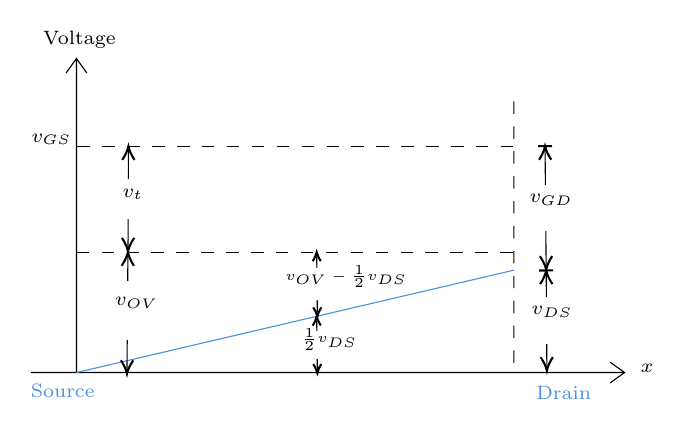
\begin{tikzpicture}[x=0.75pt,y=0.75pt,yscale=-1,xscale=1]
%uncomment if require: \path (0,300); %set diagram left start at 0, and has height of 300

%Shape: Axis 2D [id:dp16906133352548214] 
\draw  (174.67,230.63) -- (460.72,230.63)(196.62,79.33) -- (196.62,230.63) (453.72,225.63) -- (460.72,230.63) -- (453.72,235.63) (191.62,86.33) -- (196.62,79.33) -- (201.62,86.33)  ;
%Straight Lines [id:da4097719673646505] 
\draw [color={rgb, 255:red, 74; green, 144; blue, 226 }  ,draw opacity=1 ]   (196.62,230.63) -- (407.39,181.3) ;
%Straight Lines [id:da6312897459635941] 
\draw  [dash pattern={on 4.5pt off 4.5pt}]  (196.76,173) -- (407.06,173) ;
%Straight Lines [id:da6521234396527927] 
\draw  [dash pattern={on 4.5pt off 4.5pt}]  (407.39,100) -- (407.4,230) ;
%Straight Lines [id:da5804415319961403] 
\draw  [dash pattern={on 4.5pt off 4.5pt}]  (197.1,121.63) -- (407.4,121.63) ;
%Straight Lines [id:da15016612766519044] 
\draw    (221.41,174.6) -- (220.97,229.3) ;
\draw [shift={(220.96,231.3)}, rotate = 270.46] [color={rgb, 255:red, 0; green, 0; blue, 0 }  ][line width=0.75]    (6.56,-2.94) .. controls (4.17,-1.38) and (1.99,-0.4) .. (0,0) .. controls (1.99,0.4) and (4.17,1.38) .. (6.56,2.94)   ;
\draw [shift={(221.42,172.6)}, rotate = 90.46] [color={rgb, 255:red, 0; green, 0; blue, 0 }  ][line width=0.75]    (6.56,-2.94) .. controls (4.17,-1.38) and (1.99,-0.4) .. (0,0) .. controls (1.99,0.4) and (4.17,1.38) .. (6.56,2.94)   ;
%Shape: Rectangle [id:dp90804440786133] 
\draw  [color={rgb, 255:red, 0; green, 0; blue, 0 }  ,draw opacity=0 ][fill={rgb, 255:red, 255; green, 255; blue, 255 }  ,fill opacity=1 ] (215.23,186.47) -- (227.15,186.47) -- (227.15,215.14) -- (215.23,215.14) -- cycle ;

%Straight Lines [id:da5772727392049948] 
\draw    (312.38,174.6) -- (312.67,201.6) ;
\draw [shift={(312.69,203.6)}, rotate = 269.38] [color={rgb, 255:red, 0; green, 0; blue, 0 }  ][line width=0.75]    (4.37,-1.96) .. controls (2.78,-0.92) and (1.32,-0.27) .. (0,0) .. controls (1.32,0.27) and (2.78,0.92) .. (4.37,1.96)   ;
\draw [shift={(312.36,172.6)}, rotate = 89.38] [color={rgb, 255:red, 0; green, 0; blue, 0 }  ][line width=0.75]    (4.37,-1.96) .. controls (2.78,-0.92) and (1.32,-0.27) .. (0,0) .. controls (1.32,0.27) and (2.78,0.92) .. (4.37,1.96)   ;
%Shape: Rectangle [id:dp08460589981284838] 
\draw  [color={rgb, 255:red, 0; green, 0; blue, 0 }  ,draw opacity=0 ][fill={rgb, 255:red, 255; green, 255; blue, 255 }  ,fill opacity=1 ] (306.56,180.49) -- (318.49,180.49) -- (318.49,195.71) -- (306.56,195.71) -- cycle ;


%Straight Lines [id:da8557797346141001] 
\draw    (312.38,205.6) -- (312.67,228.93) ;
\draw [shift={(312.69,230.93)}, rotate = 269.3] [color={rgb, 255:red, 0; green, 0; blue, 0 }  ][line width=0.75]    (4.37,-1.96) .. controls (2.78,-0.92) and (1.32,-0.27) .. (0,0) .. controls (1.32,0.27) and (2.78,0.92) .. (4.37,1.96)   ;
\draw [shift={(312.36,203.6)}, rotate = 89.3] [color={rgb, 255:red, 0; green, 0; blue, 0 }  ][line width=0.75]    (4.37,-1.96) .. controls (2.78,-0.92) and (1.32,-0.27) .. (0,0) .. controls (1.32,0.27) and (2.78,0.92) .. (4.37,1.96)   ;
%Shape: Rectangle [id:dp6147409050215762] 
\draw  [color={rgb, 255:red, 0; green, 0; blue, 0 }  ,draw opacity=0 ][fill={rgb, 255:red, 255; green, 255; blue, 255 }  ,fill opacity=1 ] (306.56,210.55) -- (318.49,210.55) -- (318.49,223.98) -- (306.56,223.98) -- cycle ;


%Straight Lines [id:da48726851772432767] 
\draw    (422.94,181.44) -- (423.26,227.77) ;
\draw [shift={(423.27,229.77)}, rotate = 269.6] [color={rgb, 255:red, 0; green, 0; blue, 0 }  ][line width=0.75]    (6.56,-2.94) .. controls (4.17,-1.38) and (1.99,-0.4) .. (0,0) .. controls (1.99,0.4) and (4.17,1.38) .. (6.56,2.94)   ;
\draw [shift={(422.94,181.44)}, rotate = 89.6] [color={rgb, 255:red, 0; green, 0; blue, 0 }  ][line width=0.75]    (0,3.35) -- (0,-3.35)(6.56,-2.94) .. controls (4.17,-1.38) and (1.99,-0.4) .. (0,0) .. controls (1.99,0.4) and (4.17,1.38) .. (6.56,2.94)   ;
%Shape: Rectangle [id:dp5171112931088883] 
\draw  [color={rgb, 255:red, 0; green, 0; blue, 0 }  ,draw opacity=0 ][fill={rgb, 255:red, 255; green, 255; blue, 255 }  ,fill opacity=1 ] (417.14,194.43) -- (429.07,194.43) -- (429.07,216.78) -- (417.14,216.78) -- cycle ;

%Straight Lines [id:da4216630681312654] 
\draw    (422.39,121.55) -- (422.92,179.11) ;
\draw [shift={(422.94,181.11)}, rotate = 269.47] [color={rgb, 255:red, 0; green, 0; blue, 0 }  ][line width=0.75]    (6.56,-2.94) .. controls (4.17,-1.38) and (1.99,-0.4) .. (0,0) .. controls (1.99,0.4) and (4.17,1.38) .. (6.56,2.94)   ;
\draw [shift={(422.39,121.55)}, rotate = 89.47] [color={rgb, 255:red, 0; green, 0; blue, 0 }  ][line width=0.75]    (0,3.35) -- (0,-3.35)(6.56,-2.94) .. controls (4.17,-1.38) and (1.99,-0.4) .. (0,0) .. controls (1.99,0.4) and (4.17,1.38) .. (6.56,2.94)   ;
%Shape: Rectangle [id:dp47575806675174737] 
\draw  [color={rgb, 255:red, 0; green, 0; blue, 0 }  ,draw opacity=0 ][fill={rgb, 255:red, 255; green, 255; blue, 255 }  ,fill opacity=1 ] (416.7,140.15) -- (428.63,140.15) -- (428.63,162.5) -- (416.7,162.5) -- cycle ;

%Straight Lines [id:da6486338714576055] 
\draw    (221.66,123.61) -- (221.47,170.3) ;
\draw [shift={(221.46,172.3)}, rotate = 270.24] [color={rgb, 255:red, 0; green, 0; blue, 0 }  ][line width=0.75]    (6.56,-2.94) .. controls (4.17,-1.38) and (1.99,-0.4) .. (0,0) .. controls (1.99,0.4) and (4.17,1.38) .. (6.56,2.94)   ;
\draw [shift={(221.67,121.61)}, rotate = 90.24] [color={rgb, 255:red, 0; green, 0; blue, 0 }  ][line width=0.75]    (6.56,-2.94) .. controls (4.17,-1.38) and (1.99,-0.4) .. (0,0) .. controls (1.99,0.4) and (4.17,1.38) .. (6.56,2.94)   ;
%Shape: Rectangle [id:dp044555434453139475] 
\draw  [color={rgb, 255:red, 0; green, 0; blue, 0 }  ,draw opacity=0 ][fill={rgb, 255:red, 255; green, 255; blue, 255 }  ,fill opacity=1 ] (215.6,137.44) -- (227.53,137.44) -- (227.53,156.47) -- (215.6,156.47) -- cycle ;


% Text Node
\draw (296.03,177.95) node [anchor=north west][inner sep=0.75pt]  [font=\tiny]  {$v_{OV} -\frac{1}{2} v_{DS}$};
% Text Node
\draw (303.7,208.17) node [anchor=north west][inner sep=0.75pt]  [font=\tiny]  {$\frac{1}{2} v_{DS}$};
% Text Node
\draw (214.03,193.07) node [anchor=north west][inner sep=0.75pt]  [font=\scriptsize]  {$v_{OV}$};
% Text Node
\draw (414.7,197.4) node [anchor=north west][inner sep=0.75pt]  [font=\scriptsize]  {$v_{DS}$};
% Text Node
\draw (413.7,143.4) node [anchor=north west][inner sep=0.75pt]  [font=\scriptsize]  {$v_{GD}$};
% Text Node
\draw (173.72,114.33) node [anchor=north west][inner sep=0.75pt]  [font=\scriptsize]  {$v_{GS}$};
% Text Node
\draw (173.39,234.93) node [anchor=north west][inner sep=0.75pt]  [font=\scriptsize,color={rgb, 255:red, 74; green, 144; blue, 226 }  ,opacity=1 ] [align=left] {Source};
% Text Node
\draw (416.89,235.93) node [anchor=north west][inner sep=0.75pt]  [font=\scriptsize,color={rgb, 255:red, 74; green, 144; blue, 226 }  ,opacity=1 ] [align=left] {Drain};
% Text Node
\draw (467.35,225.14) node [anchor=north west][inner sep=0.75pt]  [font=\scriptsize]  {$x$};
% Text Node
\draw (179.35,64.74) node [anchor=north west][inner sep=0.75pt]  [font=\scriptsize] [align=left] {Voltage};
% Text Node
\draw (217.6,140.84) node [anchor=north west][inner sep=0.75pt]  [font=\scriptsize]  {$v_{t}$};
\end{tikzpicture}
\end{center}
以下為非嚴謹推導,因為
\end{document}
